\chapter {The Z-Wave Expert User Interface}
\label{expertuserinterface}
\label{eui}
\index{Expert User Interface}

The \zweui is designed for installers, technically savvy people, 
and other users that know how to build and maintain a \zwave-based wireless network.
Hence, it uses some \zwave specific-language and offers detailed insight into the work 
and data structure of the \zwave network. It allows users to:

\begin{itemize}
\item Add (include) and remove (exclude) \zwave devices and manage the network.
\item Configure \zwave devices.
\item Operate \zwave devices.
\item Manage Associations between wireless devices.
\item Access all data generated by the devices and perform all kind of functions and actions to the device.
\item Look behind the scene into the data structures, routing mechanisms, and timings of 
the \zwave control stack. This is particularly useful for debugging and software development.
\end{itemize}
The \zweui does not provide any access to a higher order business logic and 
automation. Please refer to the \zwshui for these functions. 
The user interface offers a home screen and five top menu items:

\begin{itemize}
\item \menu{Control}: Access to functions of the wireless devices included in the network
\item \menu{Device}: Access to information about devices
\item \menu{Configuration}: Configure the devices after inclusion if needed
\item \menu{Network}: Add and remove devices and manage the network
\item \menu{Analytics}: Allows debugging the wireless network (Please note that this mean item 
is only shown and its corresponding functions are unlocked in the transceivers firmware
\end{itemize}

Besides the menu items, there is a configuration setting (wheel icon), a time indicator 
showing the time at the time zone of the gateway and a job queue indicator. Clicking on this 
job queue indicator opens a new tab displaying the job queue of \zway. Please refer to 
Chapter \ref{jobqueue} for more information about the job queue.

All values shown in the \zweui are assigned to a time stamp indicating when 
the value of status information was received from the wireless network. A red color 
of the time stamp indicates that the update request from the controller to the device 
for this value is pending.

\begin{figure}
\begin{center}
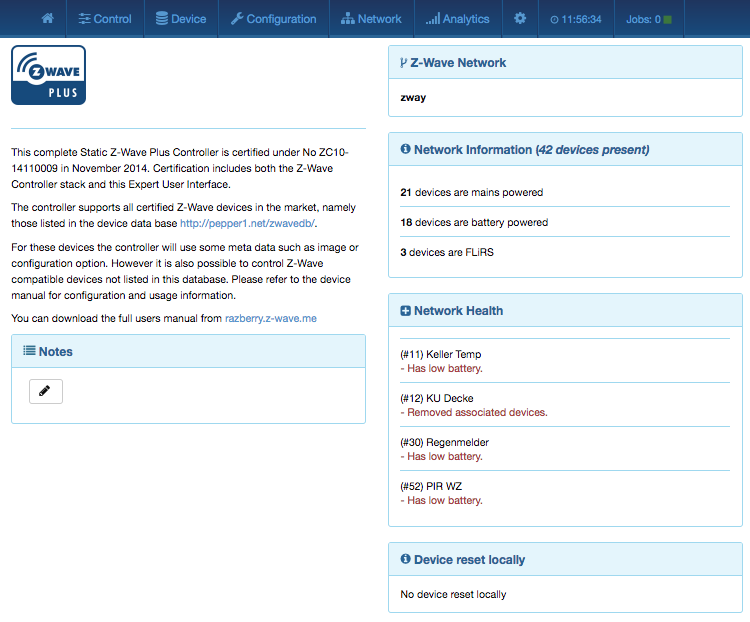
\includegraphics[width=0.8\textwidth]{pngs/cap7/eui1.png}
\caption{Sceenshot of the Expert User Interface Home Screen}
\label{eui1}
\end{center}
\end{figure}


\section{Home Screen}

The home screen shown in Figure \ref{eui1} offers some high level of information about 
the software and a notepad where the user or installer can leave important information 
for future use.

The section 'Network Information' box offers some statistics about the number of devices in 
the network and how many of them are mains or battery-operated. The network health box 
will list devices that have problems:

\begin{itemize}
\item Low battery.
\item Incomplete interview.
\item Device failed.
\item Inconsistencies on Association settings.
\end{itemize}

Clicking on the statement will lead to a help page explaining the problems and giving 
guidance for remediation.

The last infobox will contain information about devices that were removed using 
the device reset function. In this case, the device will leave the network but 
informing the controller. There is no exclusion process applied.

\section{Control}

The tab \menu{Control} allows operating the various types of device and shows the reported 
values in case of sensors or meters. In case the control options offered here are not 
sufficient, please refer to  \menu{Configuration > Expert Command}  for a full set of functions supported by the device.

\subsection{Switch}

\begin{figure}
\begin{center}
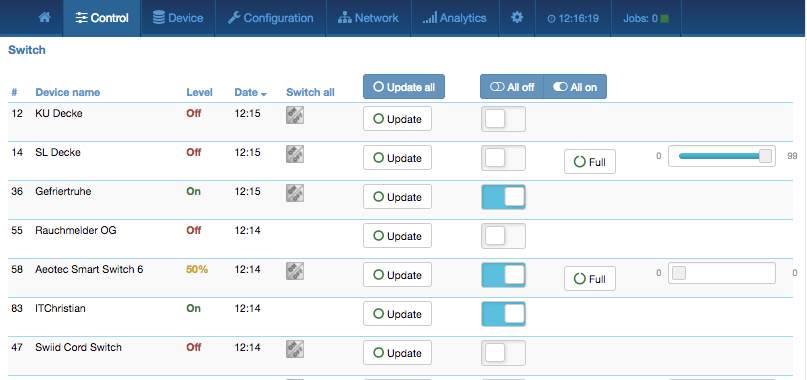
\includegraphics[width=0.9\textwidth]{pngs/cap7/eui2.png}
\caption{Control Interface for Switches, Dimmers and Motor Controls}
\label{eui2}
\end{center}
\end{figure}

The switch dialog shown in Figure \ref{eui2} lists all devices of the network supporting 
switching, dimmer, or motor control capabilities. The device name and \zwave ID, as well a 
the current status of the switch, are given and the time of the last status update. 
The \keystroke{Update} button forces an immediate update of the switch (if mains powered device). 
A 'Switch All' Icon shows whether or not the specific device will react to 
a \keystroke{All ON} or \keystroke{All Off} command. A green triangle indicates that the 
device will react to the command shown.
All actuators can be switched on or off. Dimmer and motors controls can be operated 
using a slider. For dimmer, there is a button \keystroke{On} and \keystroke{Full}. \keystroke{Full} turns the 
dimmer always to 100 \%, diming value while \keystroke{On} turns to the last dimming state
before the dimmer was turned off. Clicking on the table heads reorders the table 
view of the data.

\subsection{Sensors}

\begin{figure}
\begin{center}
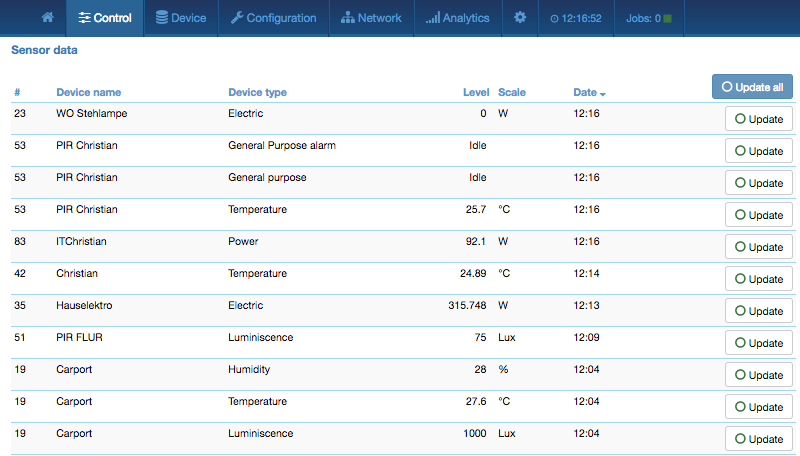
\includegraphics[width=0.9\textwidth]{pngs/cap7/eui3.png}
\caption{Control Interface for Sensors}
\label{eui3}
\end{center}
\end{figure}

The sensor dialog shown in Figure \ref{eui3} lists all devices of the network providing 
sensor information. Device name and ID, the type of the sensor, the actual sensor value 
and the sensor scale is listed. The date/time column indicates when the given sensor 
value was received. It’s possible to call for a sensor update but bear in mind that 
battery-operated device will only respond after the next wakeup.

\subsection{Meters}

\begin{figure}
\begin{center}
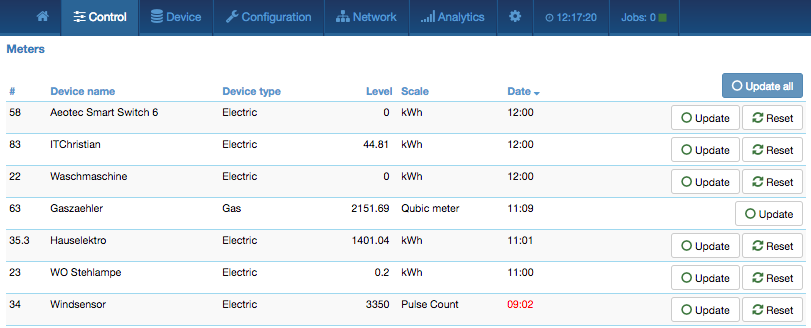
\includegraphics[width=0.9\textwidth]{pngs/cap7/eui4.png}
\caption{Control Interface for Meters}
\label{eui4}
\end{center}
\end{figure}

The meter dialog shown in Figure \ref{eui4} lists all devices of the network providing  
(accumulating) meter information.
Device name and id, the type of the meter, the actual meter value and the meter scale
 is listed. The date/time column indicates when the given sensor value was received. It’s 
 possible to call for a meter update but bear in mind that battery-operated device will 
 only respond after the next wakeup. Clicking on the table heads reorders the table 
 view of the data. A \keystroke{meter reset} button is shown for device supporting this function.

\subsection{Thermostats}

\begin{figure}
\begin{center}
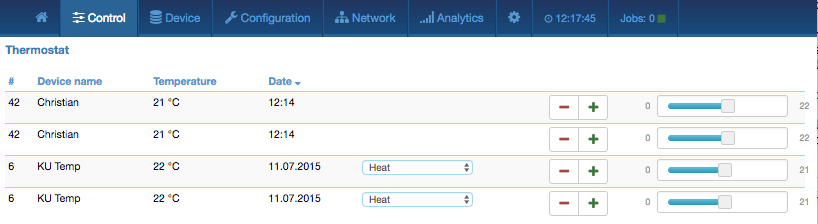
\includegraphics[width=0.9\textwidth]{pngs/cap7/eui5.png}
\caption{Control Interface for Thermostats}
\label{eui5}
\end{center}
\end{figure}

The thermostat dialog shown in Figure \ref{eui5} lists all thermostat devices of the 
network. Device name and ID and the current set point temperature is shown. The date/time 
column indicates when the given set point temperature was transferred to the device. The 
set point temperature can be changed using the \keystroke{+} or \keystroke{-} buttons or the slider. Clicking 
on the table heads reorders the table view of the data.

Some thermostats may offer different modes such as heating, cooling, off, etc. For these 
devices, a drop-down list shows all modes available. In this case, the setpoint is only 
valid for the mode selected.

\subsection{Locks}

\begin{figure}
\begin{center}
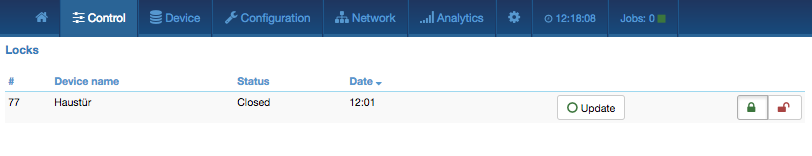
\includegraphics[width=0.9\textwidth]{pngs/cap7/eui6.png}
\caption{Control Interface for Locks}
\label{eui6}
\end{center}
\end{figure}

The door lock dialog shown in Figure \ref{eui6} lists all door lock devices of the network. 
Device name and ID, the current status of the lock, and the last time of the change of 
the status are listed. The lock can be opened or closed.
Clicking on the table heads reorders the table view of the data.

\subsection{Notifications}

\begin{figure}
\begin{center}
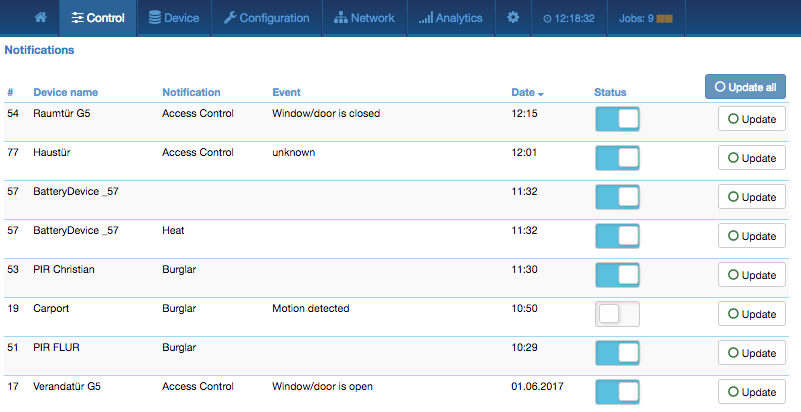
\includegraphics[width=0.9\textwidth]{pngs/cap7/eui7.png}
\caption{Control Interface for Notification Devices}
\label{eui7}
\end{center}
\end{figure}

The notification dialog shown in Figure \ref{eui7} lists all notification devices. 
Notification devices act like binary sensors, albeit offering some more capabilities. 
Per notification device multiple events can be reported. The notification device also 
allows deactivating the notification for certain events. Please note that not all 
devices make use of these functions.

\section{Device}

The menu \menu{Device} gives access to overview pages with more detailed information about 
the devices in the network and their actual status.

\subsection{Status}

\begin{figure}
\begin{center}
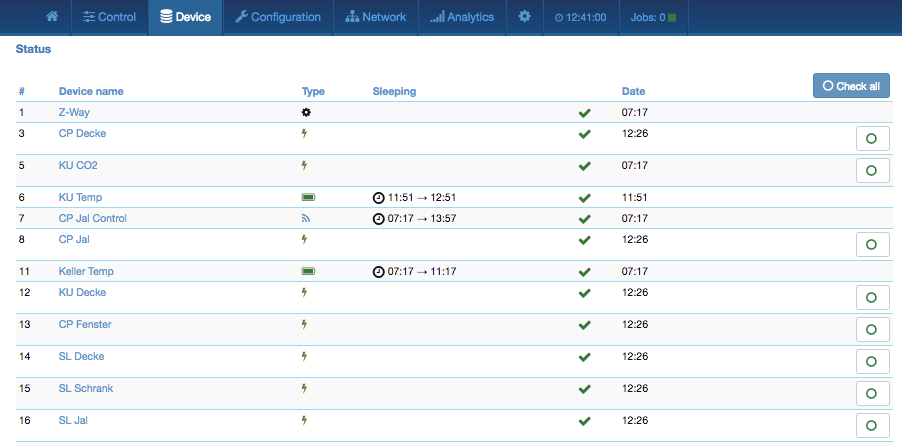
\includegraphics[width=0.9\textwidth]{pngs/cap7/eui11.png}
\caption{Device status overview}
\label{eui11}
\end{center}
\end{figure}

This dialog in Figure \ref{eui11} shows the actual network status of all devices. All 
devices are listed by their node ID and name. The date/time indicates the time of the 
last successful communications between the controller and this device (either confirmed
 sending or reception). The green checkmark indicates that the device is alive. A red 
 sign indicates that the controller assumes the device not being active anymore. Mains 
 powered devices can be checked for their network availability by hitting the \keystroke{o} 
 button on the right-hand side.

In case the device interview and configuration were not performed properly, a little 
question mark icon will indicate this. Clicking on the question mark will open a window 
displaying the details of the interview process.
The correct loading of a Device Description File\footnote{For more information about 
Device Description files, please refer to Section \ref{interview}.} is indicated as 
well. For a battery-operated device, the time of the last wakeup, the time of the 
next wakeup, and the current wakeup status are shown. Clicking on the table heads 
reorders the table view of the data. Clicking on the table heads reorders the 
table view of the data.

\subsection{Type Info}
\index{Device Types}

\begin{figure}
\begin{center}
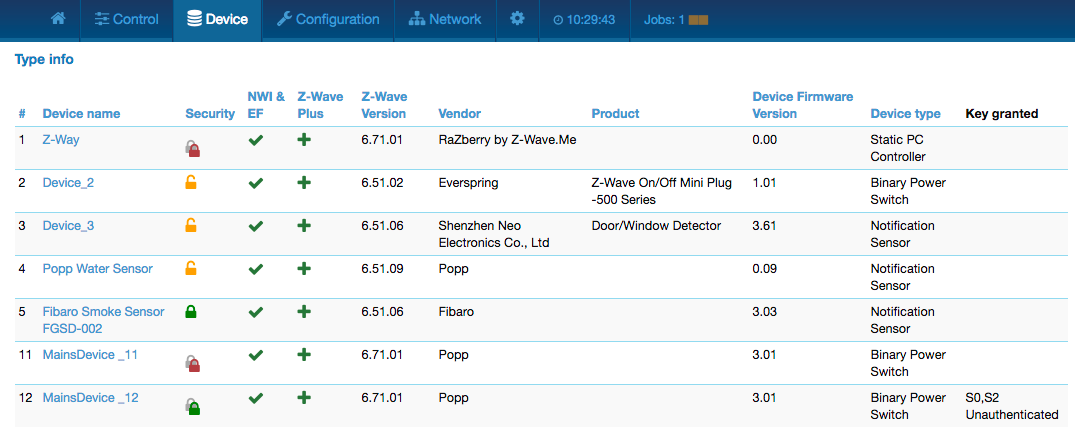
\includegraphics[width=0.9\textwidth]{pngs/security2_1.png}
\caption{Device information overview}
\label{eui12}
\end{center}
\end{figure}

The type info dialog shown in Figure \ref{eui12} lists all devices of the network and
indicates if they support enhanced \zwave functions such as Security and \zwave Plus.
Additionally, the \zwave protocol version, the application version and the device type 
indicator of the device is shown.

The security icon determines what kind of security the device supports:

\begin{itemize}
\item 
\includegraphics[width=0.04\textwidth]{pngs/cap7/s2icon1.png}: Device does not support any security class
\item 
\includegraphics[width=0.04\textwidth]{pngs/cap7/s2icon3.png}: Device supports security version 1
\item 
\includegraphics[width=0.04\textwidth]{pngs/cap7/s2icon4.png}: Device supports security version 2
\item 
\includegraphics[width=0.04\textwidth]{pngs/cap7/s2icon2.png}: Device supports security version 2 but authentication failed
\end{itemize}

The last column shows the security keys granted for the device.

Clicking on the table heads reorders the table view of the data.


\subsection{Battery}
\index{Battery}

\begin{figure}
\begin{center}
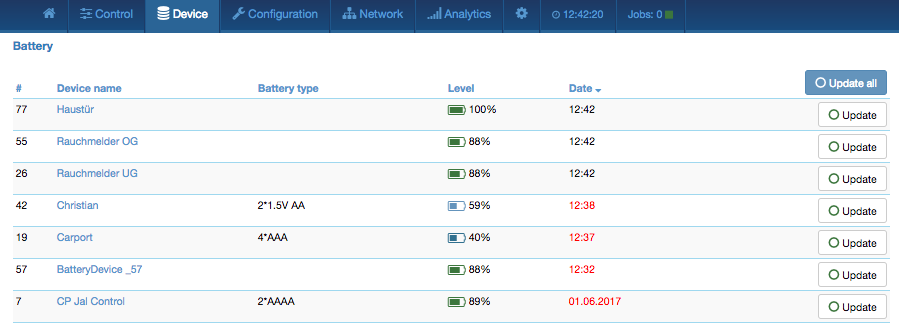
\includegraphics[width=0.9\textwidth]{pngs/cap7/eui13.png}
\caption{Battery status overview}
\label{eui13}
\end{center}
\end{figure}

This dialog shown in Figure \ref{eui13} gives an overview of the battery status of the 
battery-operated devices in the network. Devices are listed by name and id. The last 
reported battery level (0--100 \%) including update time is shown as well as the number 
and type of battery if known. The \keystroke{Update All} button will request a status update 
from the device. The new status will be available after the next wakeup of the 
device. Clicking on the table heads reorders the table view of the data.

\subsection{Active Associations}
\index{Associations}

\begin{figure}
\begin{center}
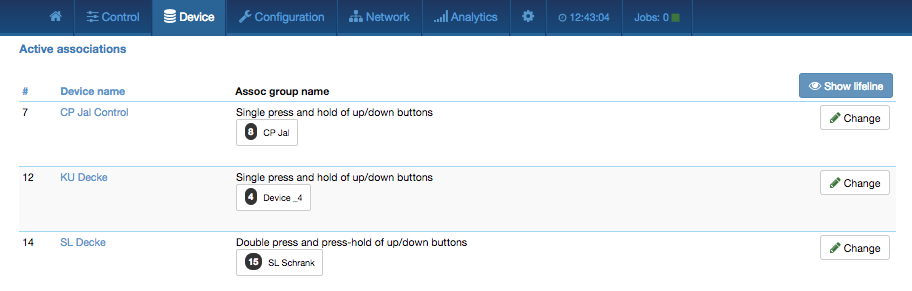
\includegraphics[width=0.9\textwidth]{pngs/cap7/eui14.png}
\caption{Active association overview}
\label{eui14}
\end{center}
\end{figure}


This overview page shown in Figure \ref{eui14} lists the current association set in the 
network. The Lifeline is an association to the gateway to report status changes and heard 
beat and can be hidden if needed. A \keystroke{Change} button leads right to the configuration 
page of the device to change association settings.

\section{Configuration}
\label{Configuration}
\index{Configuration}

The tab \menu{Configuration} allows configuring the functions of a particular device. Pick 
the device to be configured from the drop-down list or pick the device from the full list 
shown on the left-hand side. The functions of the device are grouped into 6 tabs.

\subsection{Interview}
\label{interview}
\index{Interview}

\begin{figure}
\begin{center}
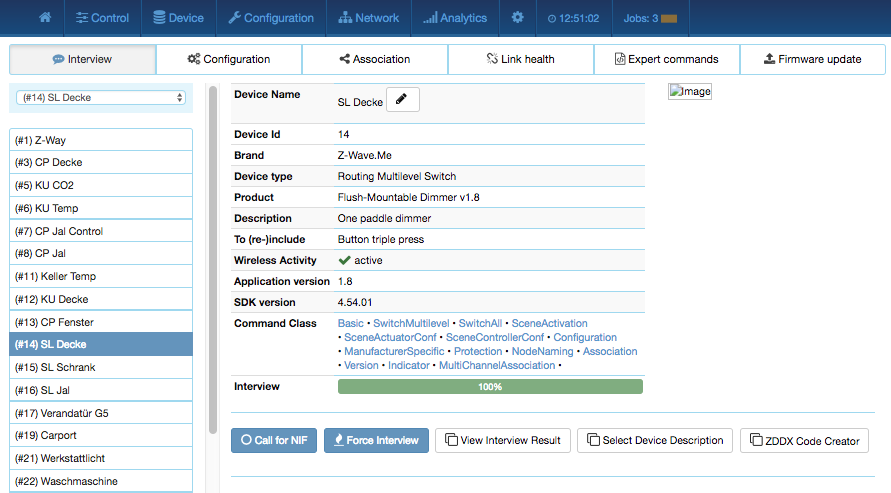
\includegraphics[width=0.9\textwidth]{pngs/cap7/eui31.png}
\caption{Device interview}
\label{eui31}
\end{center}
\end{figure}

\menu{Configuration > Interview}, as shown in Figure \ref{eui31}, documents the result of 
the device interview. In this process, the controller tries to get information about the 
device. In case the controller finds a device description record for the device, it 
will display further information about the device that cannot be obtained from the device itself:

\begin{itemize}
\item Product Image
\item Information regarding how to include the device
\item Information for battery-operated devices about how to wake them up manually
\item Human-readable meanings of configuration parameters and values
\end{itemize}

If the software will not automatically recognize the device and load the description 
record a button \keystroke{Select Device Description Record} allows doing this manually. However, 
the description file must be present. Chapter \ref{newddr} gives further information on 
how to create an own Device Description Record and load it into \zway.

The interview stage line gives information about the progress of the device interview.

There are a few reasons why an interview is not complete: In most cases the devices went 
to deep sleep too early to have some wireless connectivity problems. The 
button \keystroke{Force Interview} allows re-doing the whole interview. The button \keystroke{Call for NIF} 
requests a Node Information Frame from the device and the Button \keystroke{View Interview Result} 
allows displaying the information about the different command classes found during the 
interview. It is also possible to force the interview of a certain command class only.

The button \keystroke{ZDDX Code Creator} allows creating an XML description file usable for 
certain device databases.

The only configuration option on this tab is to change the given name of the device. 
During inclusion, the software generates a generic name, but it is highly recommended 
to change this name. The given name should be descriptive but not too long.

\subsection{Configuration}
\index{Configuration}

\begin{figure}
\begin{center}
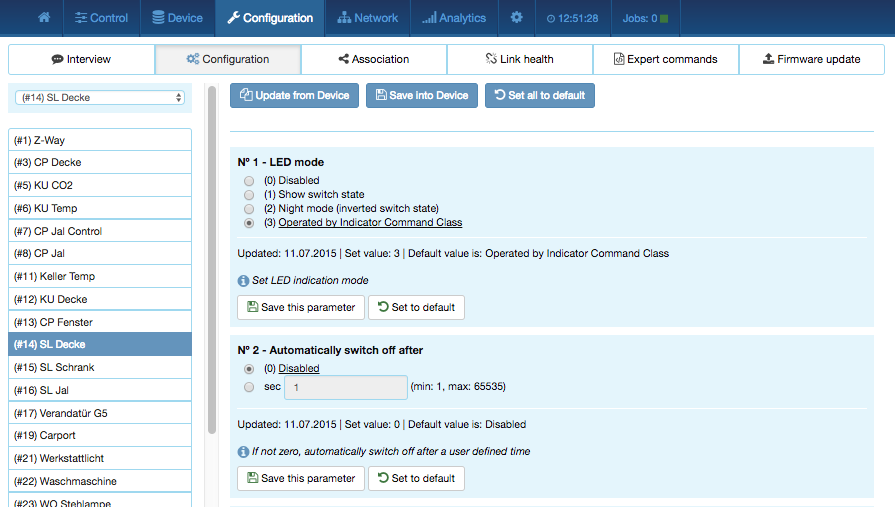
\includegraphics[width=0.9\textwidth]{pngs/cap7/eui32.png}
\caption{Configuration - convenient view}
\label{eui32}
\end{center}
\end{figure}

\menu{Configuration > Configuration} shown in Figure \ref{eui32} allows configuring the device. If the 
specific device was recognized correctly the different configuration values are translated 
into human-readable dialogs. Every configuration comes with standard dialog options:

\begin{itemize}
\item Time Stamp, when the configuration value was last updated
\item Set Value as integer
\item Information about the default value of this particular parameter
\item Button to reset to default value given by the device itself
\item Button to save the parameter into the device
\end{itemize}

If the device is not known (means there is no Device Description File assigned to it) it 
is still possible to set configuration values. Figure \ref{eui33} shows the generic 
configuration dialog used in this case. The specific configuration parameters and 
its values need to be read from the device manual.

\begin{figure}
\begin{center}
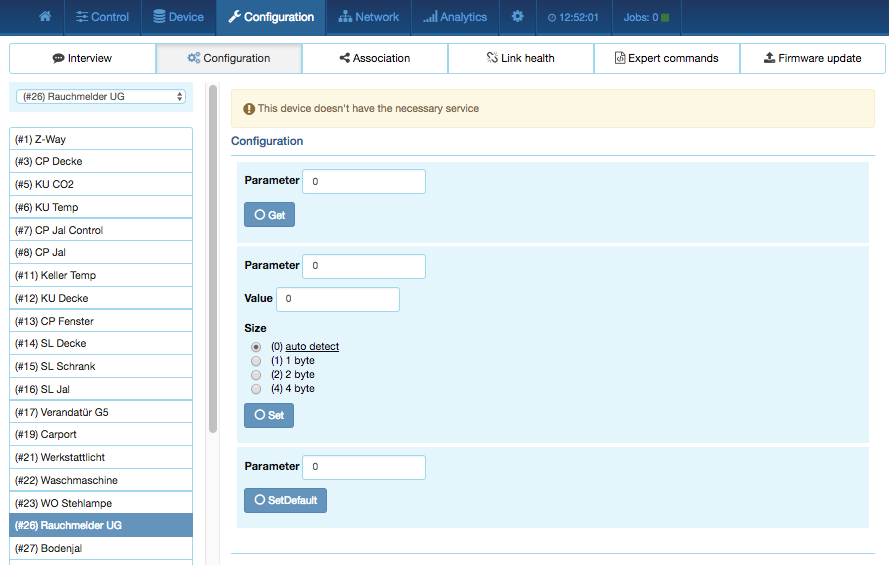
\includegraphics[width=0.9\textwidth]{pngs/cap7/eui33.png}
\caption{Configuration - generic view}
\label{eui33}
\end{center}
\end{figure}

There are four more command classes that may need additional configuration and are 
displayed in the same dialog if the device supports them.

\begin{itemize}
\item Wakeup: Define the wakeup interval and the node is of the main controller taking 
care of the wakeup sequence. The controller will set a standard wakeup time of 1800 
seconds unless the devices sets a different minimal or maximal wakeup time. In most 
cases the node ID of the controller is the correct setting for the target node ID and 
should not be changed. In case this controller is only a secondary controller, this 
value may change. A tool tip on the input field shows the allowed minimum and maximum 
wakeup time as reported by the device.
\item Protection: In case the device supports local protection, meaning suppressing 
local use of the device, the behavior of this function can be defined. The protection 
command class offers more options than displayed here. Refer to the \menu{Configuration > Expert Commands} 
tab for a complete set of controls.
\item Switch All configuration: \zwave supports the so-called switch all function as 
a broadcast to all switches and dimmers. This setup defines the reaction of the device 
to such a \keystroke{Switch All} command. The setting is also displayed in the \menu{Control > Switches} 
section as little gray/green icon.
\end{itemize}

Note: For mains-powered and FLIRS devices, the button \keystroke{Save this parameter} or
 \keystroke{Save into Device} will activate the changes within few seconds. For battery-operated 
 devices, the commands are stored to the next wakeup. It’s possible and recommended to 
 wake up the device manually to speed up the change of configuration values.

\subsection{Association}
\index{Association}

\begin{figure}
\begin{center}
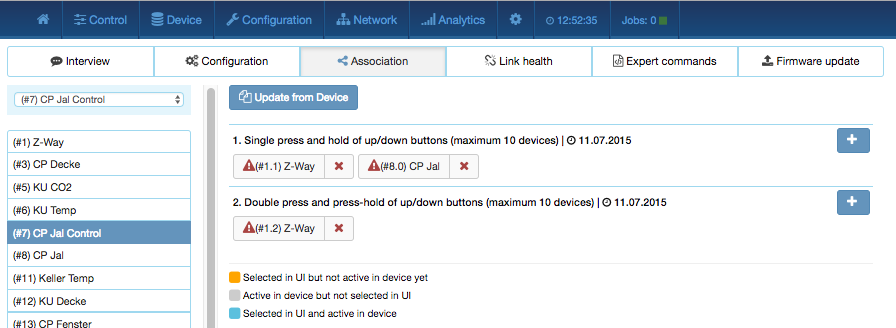
\includegraphics[width=0.9\textwidth]{pngs/cap7/eui34.png}
\caption{Association dialog}
\label{eui34}
\end{center}
\end{figure}

Associations allow switching a \zwave Device B (target) as a result of an event in 
\zwave Device A (source). \zwave Device A manages a list of devices to be controlled for 
each event supported. The device list associated to a specific event---also called 
association groups---and the devices that are associated with it are shown in the 
association tab in Figure\ref{eui34}.

In case the information is provided either by the device or by the device record 
stored in the software, the meaning of the events is written. Otherwise, the 
event group is shown unnamed as number only. In this case, refer to the devices 
manual for more information about the association group meaning.


The stored devices can be called from the actual device using a button. The buttons \keystroke{+/-} 
used to add and remove device from the group. A dialog is opened and a device can be picked. 
In case this device has multiple instances, an instance drop-down list will appear allowing 
to choose the right instance of the target device. The node ID and---if applicable---the 
instance ID are shown in the target device list. Move the mouse over the ID to show the 
complete given name of this device. The color of the device name or ID indicate the status 
of the association entry:

\begin{itemize}
\item Yellow: Selected in user interface but not stored in device.
\item Grey: Active in device but not selected in user interface.
\item Blue: Selected in user interface and stored in device.
\end{itemize}

\subsection{Link Health}
\index{Link Health}

\begin{figure}
\begin{center}
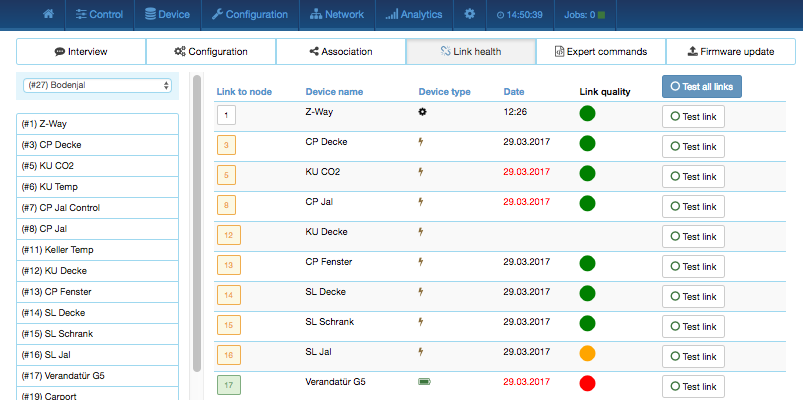
\includegraphics[width=0.9\textwidth]{pngs/cap7/eui36.png}
\caption{Link health}
\label{eui36}
\end{center}
\end{figure}

Modern versions of \zwave allow testing the quality of a link between two devices in 
direct wireless range. The dialog shown in Figure \ref{eui36} lists all devices in 
wireless range and gives an indication about the quality of this link. The following 
colors are used:

\begin{itemize}
\item grey: untested
\item green: good quality
\item yellow: reasonable quality
\item red: link quality insufficient
\end{itemize}

Individual links can be retested using the \keystroke{Test all links} button. It is also possible to 
test all links from a given device. However, please keep in mind that this process may 
take several minutes to complete.


\subsection{Expert Commands}

\begin{figure}
\begin{center}
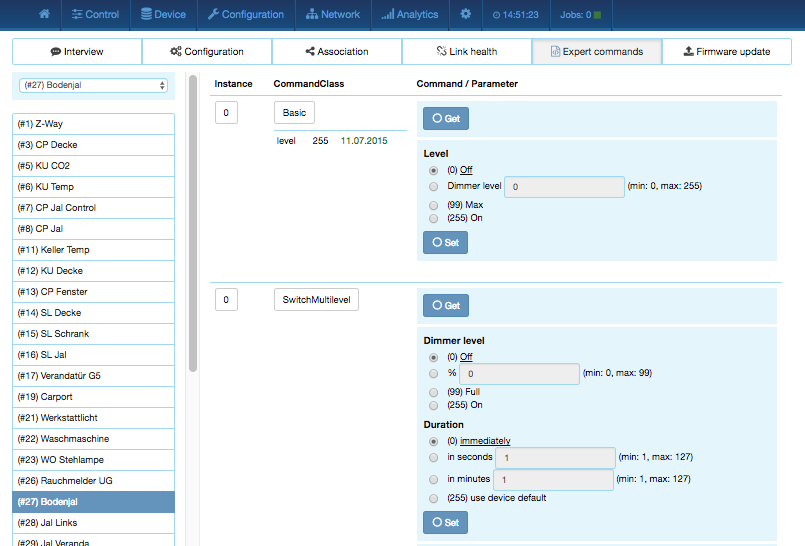
\includegraphics[width=0.9\textwidth]{pngs/cap7/eui35.png}
\caption{Experts commands}
\label{eui35}
\end{center}
\end{figure}

\menu{Configuration > Expert Commands } as shown in Figure \ref{eui35} displays the status values and 
possible commands in a very generic way. On the left-hand side, the different instances 
(channels) of the device are listed in a column. In case there is only one channel (that’s 
the case for most devices), only channel/instance 0 is shown. Clicking on the number 
opens a dialog showing all internal variables for the channel. The next column shows all 
the command classes exposed by the device. Again, clicking on the name opens a dialog with 
more internal status variable information for this command class.
On the right-hand side, there is a list of commands. This dialog form is auto-generated 
from the information provided by the command class itself and not optimized for daily usage.


\subsection{Firmware Update}
\index{Firmware Update}

In case the device supports a firmware update ``over the air,’’ this dialog is shown to 
perform such a firmware update.  The firmware file to be uploaded must be available in a 
raw ``BIN’’ or the Intel hex ``HEX’’ file.
The target field allows specifying the target memory/processor for the update process. 
For updating the \zwave firmware part a ``0’’ must be set. The firmware updating process 
will take up to 10 minutes. Please don’t do any other operation during this time.
It may be required to activate the firmware update mode on the device to be updated. 
Please refer to the manual for further information about activation.


\section{Network}

The network section of the user interface focuses on the network as such and offers all 
controls and information to build, manage, and repair the wireless network of the controller.

\subsection{Control}

\menu{Network > Control} summarizes all commands needed to manage the network and the controller.
The page is structured in four boxes.

\subsubsection{Device Management}

\index{Inclusion}
\index{Exclusion}

\begin{figure}
\begin{center}
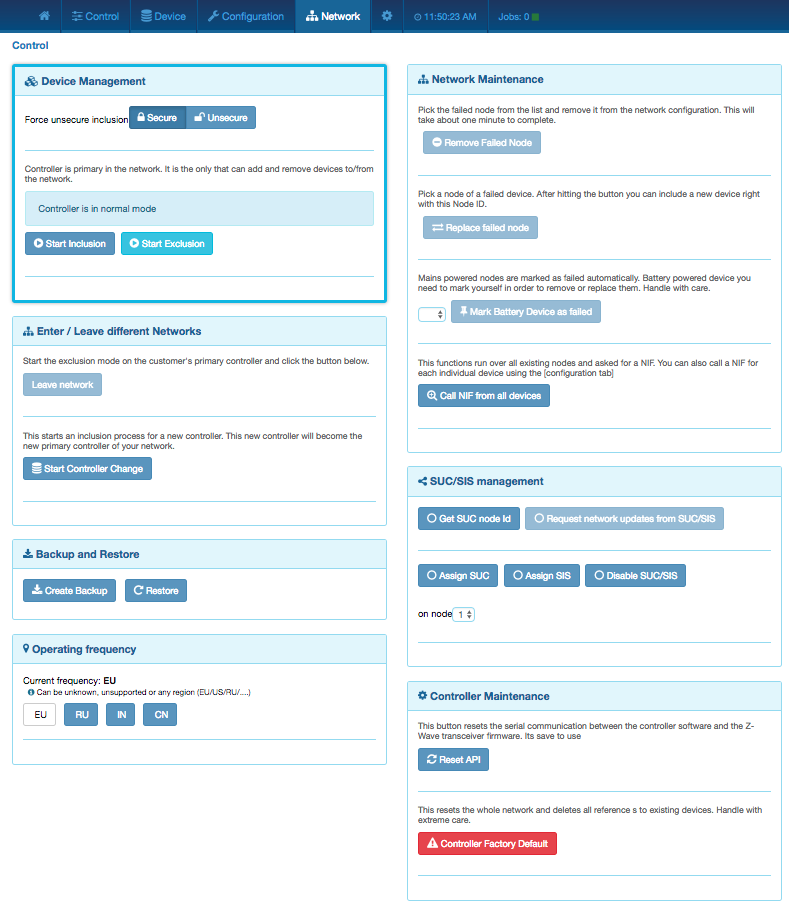
\includegraphics[width=0.9\textwidth]{pngs/cap7/eui21.png}
\caption{Network Management}
\label{eui21}
\end{center}
\end{figure}

The device management box as shown in Figure \ref{eui21} allows including and excluding 
\zwave devices. A status display shows the status of the controller. The \keystroke{Include Device} 
and \keystroke{Exclude Device} button turn the controller into the Inclusion and Exclusion mode. In 
this case the status display changes and the resp. buttons turns into a \keystroke{Stop} function. 
The inclusion and exclusion modes will time out after about 20 seconds but can always be 
terminated using the \keystroke{Stop} buttons.

Another way to stop the inclusion mode is to actually include a new device. In this case
 the inclusion mode will stop and the node ID of the new device is shown. The controller 
 generated a default name of the device as combination of its primary function and the 
 new node ID. Clicking on this default name leads to the \menu{Configuration} page where the 
 name can be changed and other configuration tasks can be performed.

\textbf{Please refer to the devices manual on how to do an inclusion. In case the 
inclusion does not work as expected, please exclude the device first. More than 90 \% of 
all inclusion problems are caused by still included in a different network and can then 
not being included again.}

The Exclusion mode also stops when one device was successfully excluded. This function 
can exclude devices from other networks too but the device need be available and 
functioning. To remove nonfunctioning or disappeared devices please refer to 
\keystroke{Replace Failed node} or \keystroke{Remove Failed node.}

In case the new device supports enhanced security function (Security Command Class), this 
controller will include the device securely. After this all data exchange between the 
controller and the new device is encrypted using AES encryption. For performance reasons, 
it mays be desired not to use the security function. The slider \keystroke{Force unsecure inclusion} 
turns the controller into a mode where all security functions are suppressed for the included 
device. Security functions of other devices are not impacted. In case the new device supports 
Security S2 right after inclusion, a pop-up window will appear asking the user to grant the 
S2 security keys.
A few basics about this process: Security in \zwave means among others that all 
communication between two nodes over the air is encrypted. Encryption however requires 
a key to encrypt and all the device communicating shall have the very same key---usually 
called network key. \zwave Security 2 handles 4 different network key. They differ by 
their level of trust.

\begin{itemize}
\item S0:The network key is needed to communicate with a device capable of Security CC 
Version 1. Hence, this is more for backward compatibility.
\item S2 Unauthenticated: The device-specific key of the device included is not verified. 
In case the device has its key (as PIN number of QR Code) on the enclosure, it is possible 
to compare the two numbers but the key assignment does not verify this choice.
\item S2 Authenticated: Right after inclusion, the device-specific key (as a PIN or AR code) 
must be manually provided to the included controller in order to verify the identity of the device just included.
\item S2 Access Control: This key requires similar authentication than S2 authenticated.
 This additional key is provided to separate control of door locks and other access devices from other devices.
\end{itemize}

\begin{figure}
\begin{center}
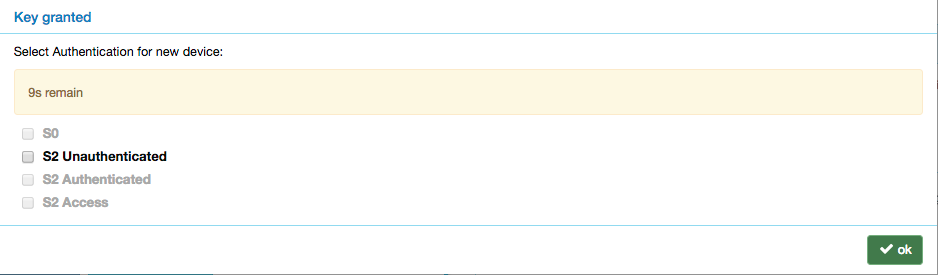
\includegraphics[width=0.9\textwidth]{pngs/cap7/security2_2.png}
\caption{\zweui - S2 key selection}
\label{security2_2}
\end{center}
\end{figure}

Each device will request one of more network keys according to the device 
usage and implementation idea. The default key is likely  S2 Authenticated but Door Locks 
will ask for S2 Access control and small devices without external label request S2 
Unauthenticated only. Figure \ref{security2_2} shows the dialog to grant the keys. The 
requested key is displayed in bold letters. The user has 20 seconds to select the keys to be granted.
If no selection is made with 20 seconds, the process will time out and the device is 
included unsecure. Please note that some devices may still offer valid functions 
while other will deny any function outside a secure environment. It is recommended 
to grant the keys requested, but there may be certain environments where other 
selections may make sense.

\begin{figure}
\begin{center}
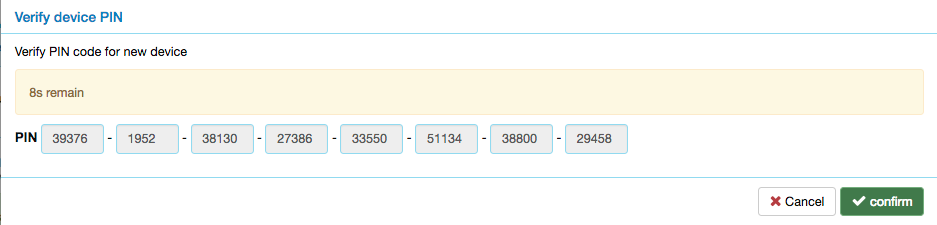
\includegraphics[width=0.9\textwidth]{pngs/cap7/security2_3.png}
\caption{\zweui - S2 key display}
\label{security2_3}
\end{center}
\end{figure}


Once the selection is made before timeout a second window  will request 
the authentication of the device. In case of S0 or S2 Unauthenticated, the window 
displays the device-specific key for information only as shown in Figure \ref{security2_3}. 
If a key is visible on the device, it is recommended to compare the numbers. However, 
the key is granted without any further interaction by the user.

\begin{figure}
\begin{center}
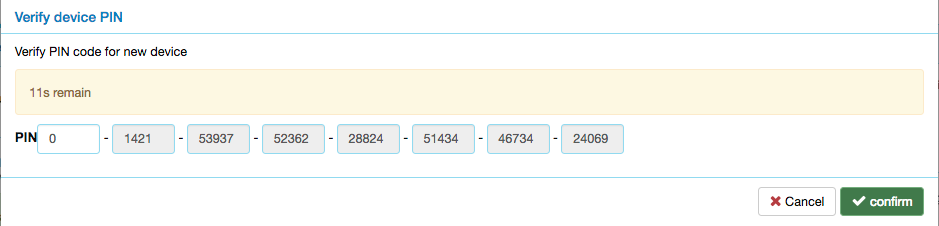
\includegraphics[width=0.9\textwidth]{pngs/cap7/security2_4.png}
\caption{Expert User Interface - S2 authentication}
\label{security2_4}
\end{center}
\end{figure}


In case S2 Authenticated or S2 Access Control keys were requested the 
dialog windows asks for providing the Device information by the user. This can be done 
by typing in the 5-digit PIN code (first 5 numbers of the device-specific key) as shown
in Figure} \ref{security2_4} or by 
scanning the QR code on the device shown in Figure \ref{security2_5}.

In case of Access or Authentication, the user must insert either a PIN 
number or scan a QR code from the device just included. This insures 100\% that the device 
just included is really the device in hand.
If authentication fails, an error message is displayed. It is not possible to redo 
the key authentication only. You must exclude and re-include the device.


\subsubsection{Smart Start}

Smart Start is a new way to include devices into Z-Wave using the QR code provided with S2
authentication.  The user scans the QR code thats is stored in an internal so called 
provisioning list. Smart Start Devices will then announce to be included when powered up.
In case the S2 key is in the provisioning list the controller will automatically include 
this new device without any further user interaction.

Smart Start is controlled by the button} \keystroke{Activate/Deactivate Smart Start.
The button \keystroke{Smart Start} opens a submenu allowing to register Device keys either 
by typing the 8 groups of numbers as shown in Figure \ref{ss1} or using 
a QR code scanner as shown in Figure \ref{ss2}. Please note that a standard
web browser running on a standard PC may not provide the capability to scan QR codes.

\begin{figure}
\begin{center}
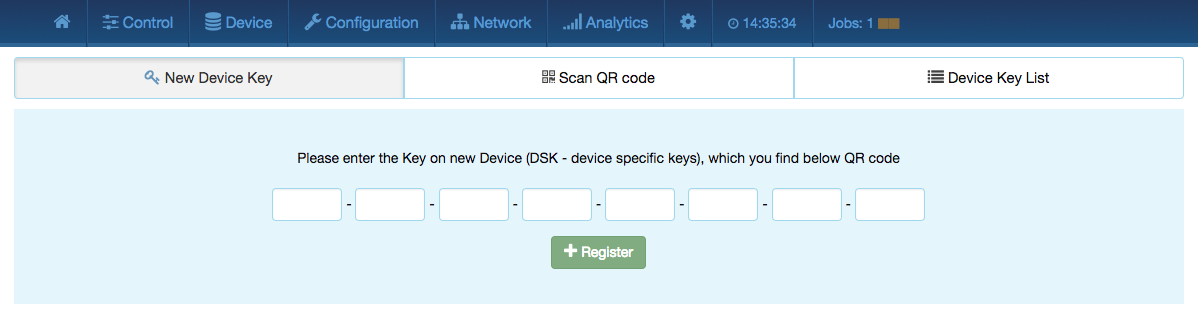
\includegraphics[width=0.9\textwidth]{pngs/cap7/ss1.png}
\caption{Smart Start - enter Device Key (DSK)}
\label{ss1}
\end{center}
\end{figure}

\begin{figure}
\begin{center}
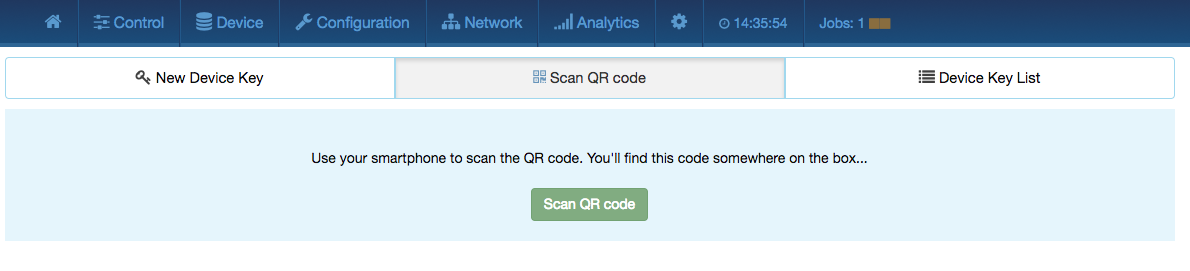
\includegraphics[width=0.9\textwidth]{pngs/cap7/ss2.png}
\caption{Smart Start - scan QR code (on smart phones only}
\label{ss2}
\end{center}
\end{figure}

\begin{figure}
\begin{center}
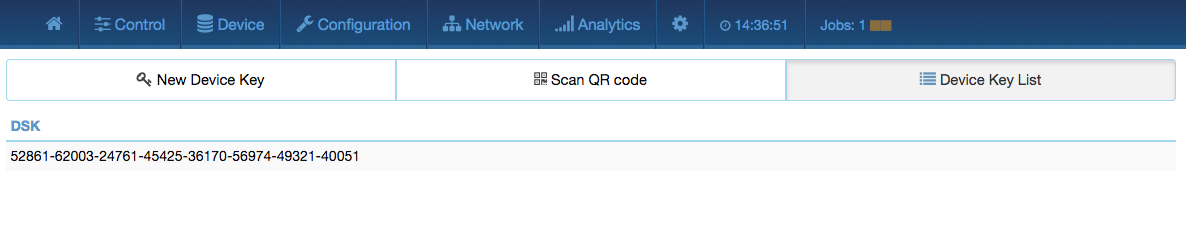
\includegraphics[width=0.9\textwidth]{pngs/cap7/ss3.png}
\caption{Smart Start Provisioning list}
\label{ss3}
\end{center}
\end{figure}

Figure \ref{ss3} finally shows the lost of Device keys already registered 
in the system and not used. Used means in this context that the corresponding device
was powered up in proximity of the controller and got included automatically. Please note that
the Razberry Shield or UZB or any hardware used must provide a firmware with SDK >=6.81. 
Otherwise Smart Start will not work.



\subsubsection{Enter/Leave different Network}


This button will only be active if \zway is in factory default state. Only in this case 
the controller can be added to a different network as secondary controller. The controller 
of the other network must be in either the Inclusion or in the Exclusion mode, and the 
Learn button confirm the process.


\begin{figure}
\begin{center}

\includegraphics[width=0.5\textwidth]{pngs/cap7/security2_5.png}
\caption{\zway -  own key for authentication}
\label{security2_5}
\end{center}
\end{figure}

In case the new primary controller supports Security S2 a dialog window 
will pop up right after finishing the inclusion by the new controller. This dialog window 
will show \textbf{the PIN number and the QR Code of this \zway controller} needed to authenticate 
against the new controller.


The \keystroke{Start Change Controller} function actively hands over the role of the primary controller 
of the network to a controller that will be included using the normal inclusion process. 
The controller status dialog shows the mode and its termination.


\subsubsection{Backup and Restore}
\label{BackupandRestore}
\index{BackupandRestore}

The next dialog  box of the page allows creating and using a backup.  The backup file is 
stored on the local computer. Please note that any restore will overwrite the existing 
network. The restore operation must therefore be confirmed in another message box. A 
checkbox defines if the node information in the \zwave chip itself will be overwritten 
as well. This operation result in a possible loss of all network relationships and may 
require a re-inclusion of devices. Handle with care!

\subsubsection{Controller Maintenance}

The controller maintenance offers two reset buttons. The \keystroke{Z-Wave Chip Reboot} restarts 
the operating system of the \zwave transceiver chip. This can be done safely all the time.

The \keystroke{Reset Controller} turns the controller back into factory reset. All connections 
to included devices and all configurations and settings are lost. This function must be 
handles with extreme case. An additional dialog requires to explicitly confirm the 
function. Only use this function if you know what you do!

\subsubsection{Operating Frequency}
\index{Frequency}


This dialog allows changing the operating frequency. Please note that a wrong frequency 
will block all \zwave traffic and make the device inoperable.  Frequencies can only be 
changed within one frequency group. These are the frequencies shown side by side (e.g. 
EU, RU, IN, ...). Changing to a frequency outside this group will technically work but 
the wireless range will be few centimeters only. Hence, this for workbench testing only. 
The device will reboot after a frequency change so please allow some time for restart.

\subsubsection{Network Maintenance}

The function \keystroke{Remove Failed Node} allows removing a node that is no longer communicating 
with the controller. After multiple failed communications with a device the controller 
will mark this device as failed and avoid further communication. This function finally 
removes such a device from the network configuration. The drop-down list will only show 
IDs of failed nodes. If this list is empty this is a good sign!

It is also possible to \keystroke{Replace a Failed node} with a new node. This is a combination 
of removing the failed node and adding a new node. Using this function makes sure the next 
included node has the same node ID as the failed node. The drop-down list will only show 
IDs of failed nodes. If this list is empty this is a good sign! Battery-operated devices 
are mainly in deep-sleep state and will not answer to communication requests. Hence, the 
controller will never automatically detect if a certain device is defect or gone. The 
function \keystroke{Mark battery device as failed} manually marks battery-operated devices as 
failed so that they can be removed or replaced. The drop-down list shows all battery-operated 
devices but this does not mean that they are failed.

The \keystroke{Request NIF from all devices} function is just a convenient way to retrieve a Node 
Information Frame from all devices of the network.

\subsubsection{SUC/SIS Management}

The SUC/SIS Management pane allows manipulating the self-organization of the \zwave network. 
Don’t use this unless you are a developer who knows when and why this is needed for testing purposes.

\subsection{Neighbors}

\begin{figure}
\begin{center}
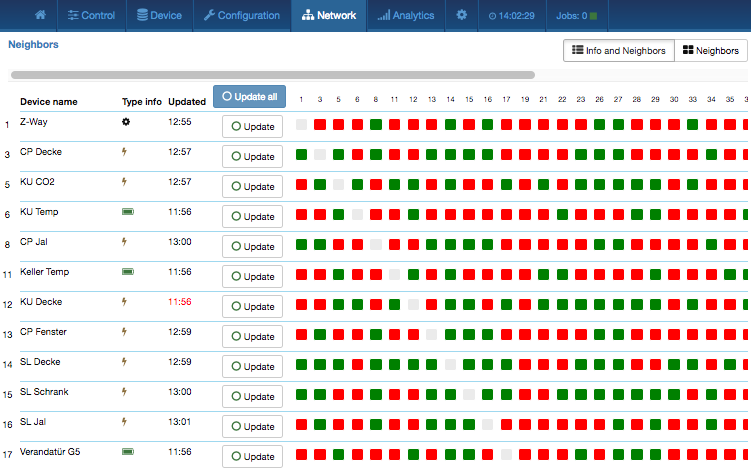
\includegraphics[width=0.8\textwidth]{pngs/cap7/eui22.png}
\caption{Neighbors}
\label{eui22}
\end{center}
\end{figure}

This table in Figure \ref{eui22} shows the neighborhood relationship of devices. The id,
 the name and the type of the node are listed. Green indicates that the two devices are 
 in direct wireless neighborhoods and don’t need any other device to forward their signals.  
 A red color between two nodes indicated that routing is needed between these devices.  
 The \keystroke{Update} button calls the device to scan its neighborhood and report back the 
 result to update its own line of the routing table.

\subsection{Reorganization}

\begin{figure}
\begin{center}
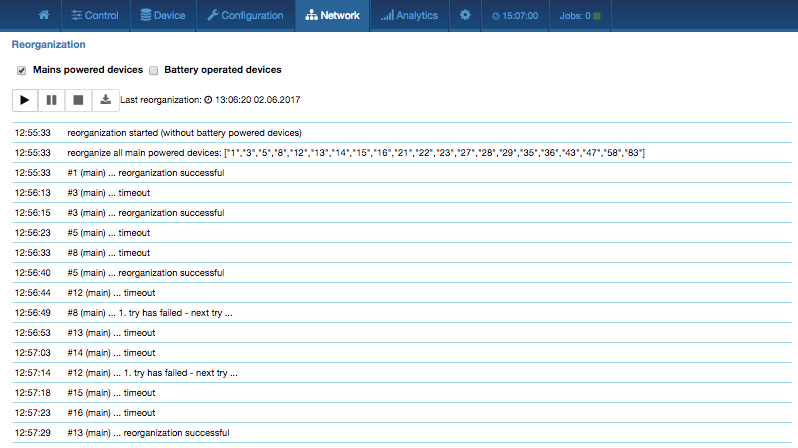
\includegraphics[width=0.9\textwidth]{pngs/cap7/eui23.png}
\caption{Reorganization}
\label{eui23}
\end{center}
\end{figure}

The reorganization page controls as shown in Figure \ref{eui23} an algorithm that 
reorganizes the network relationships and fixes problems. With checkboxes various stages 
of the algorithm can be selected. The result of the reorganization is shown in a log and 
can be downloaded. The network reorganization calls for every node to redetect its neighbors. 
This operation will work if there is a working route to this device and this device is 
not sleeping. If the operation fails, the algorithm will have three more attempts to 
reflect possible routes to the very device that may be reestablished during the 
reorganization. Detection of neighbors for battery-operated devices will be started after 
all mains-operated devices are processed. The requests to battery-operated devices will 
be queued. For more information about job queuing, please refer to Chapter \ref{jobqueue}.

\subsection{Network Map}

The \textbf{Poltorak-Chart} as a way to map the network is an extremely powerful, informative but the same time very complex
viewgraph of the network situation in a home.  The chart visualizes the possible links between
the nodes and how they are used. If provided by the devices the chart will furthermore show
complete routes and the signal strength of the individual links of a route. However only 
devices with SDK greater or equal to 6.71 will provide this additional information.
 
Initially all nodes are displayed with equal distances. It is possible to drag and drop
the nodes to match the distances between them with the real distances. This will always 
work quite well if the Z-Wave network is in one floor only. 
A 2D map can be uploaded as background image to support the mapping.
If the network is distributed  on multiple floors it is recommended to do a best guess 
to keep the round initial view.

Figure \ref{c5:poltos} shows a typical chart. By clicking on a certain node and then 
moving the mouse over it again, it is possible to analyse the traffic from and to this 
very node. This allows focusing on the situation of this node only.

\begin{figure}
\begin{center}
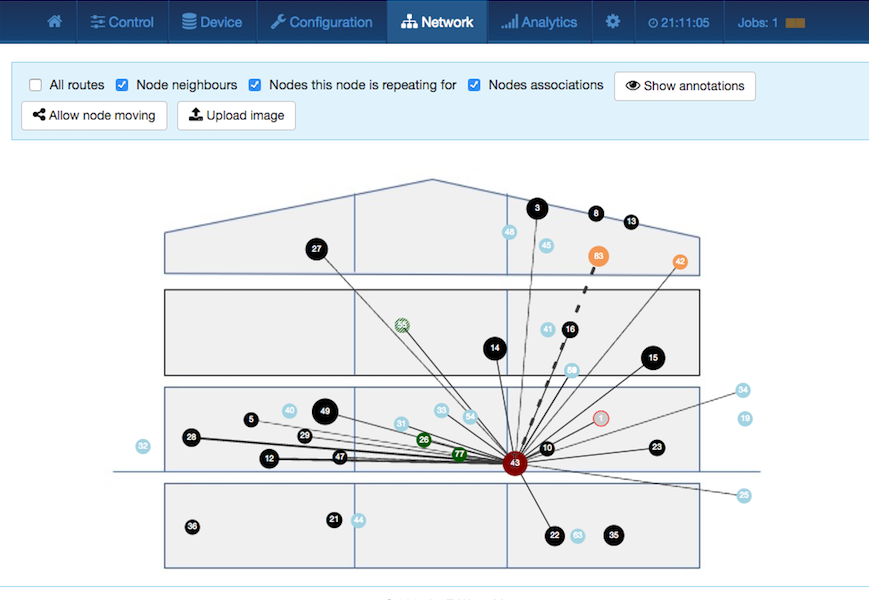
\includegraphics[width=1.0\textwidth]{pngs/cap7/eui24.png}
\caption {Poltorak-Chart}
\label{c5:poltos}
\end{center}
\end{figure}

The lines between the nodes represent the wireless connections and the communication between
the nodes. The following information is encoded in these lines:

\begin{itemize}
\item Color: The color indicates the wireless signal strength of the connection if it can be
measured. Red means a very high wireless signal.
The device is likely very closed or in direct sight of the each other. A black color means a
standard wireless strength, gray indicates that the received signal strength (RSSI value) 
is not known.

\item Thickness: The Thickness of the line indicates the amount of traffic running over
this line. This can be direct communication between the two links or routed traffic. If a 
route exist there will be a single pixel line. Every line thicker than a pixel shows real 
traffic.

\item Dotted versus solid: A dotted line indicates that this link is sometimes just not working.
\end{itemize}


\subsection{Timing Info}

\begin{figure}
\begin{center}
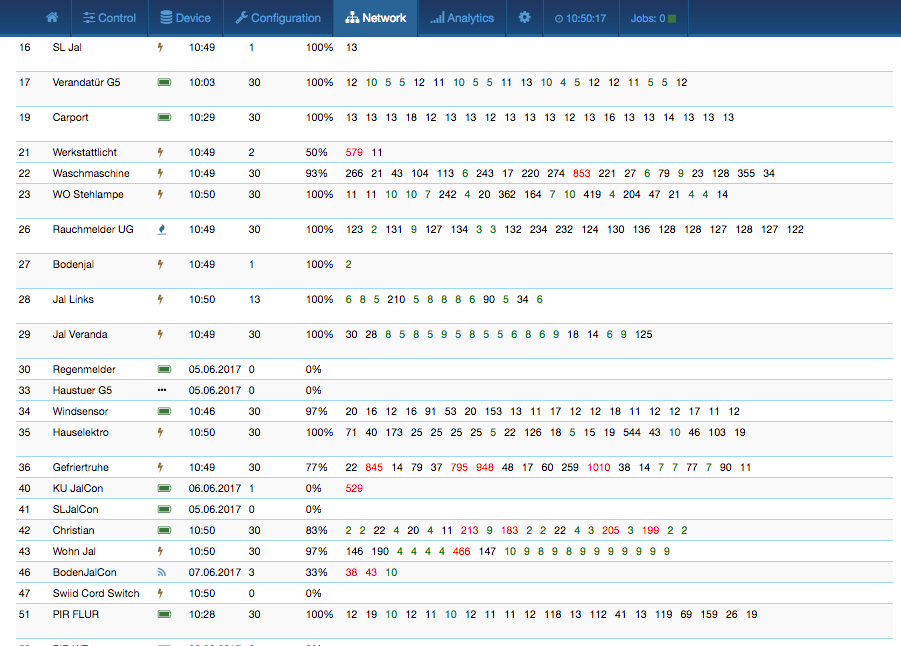
\includegraphics[width=0.9\textwidth]{pngs/cap7/eui25.png}
\caption{Timing Info}
\label{eui25}
\end{center}
\end{figure}

The Timing tab in Figure \ref{eui25} shows some very valuable timing information of 
communications between the controller and other devices. All other devices the controller 
has communicated with are shown in a list. The number of packets and the percentage of 
successful communication are shown. This can give an indication about the stability of 
the communication link between the controller and this device. On the right-hand side, 
the timing delay of each communication is shown and color-coded. A red number indicates 
that this communication finally failed. A communication without rerouting attempts as 
shown as green and a rerouting attempt is coded in black. The fact that a communication 
failed (red) may indicate that there is a severe problem in the network or in the device. 
It is however also possible that a battery-operated device just went back to sleep too fast. 
\zwave professionals can read a lot out of this timing information particularly when combined 
with the routing table. Please refer to Chapter \ref{c5:cit} for more details on 
troubleshooting \zwave networks.


\subsection{Link Status}
\index{Link Health}


\begin{figure}
\begin{center}
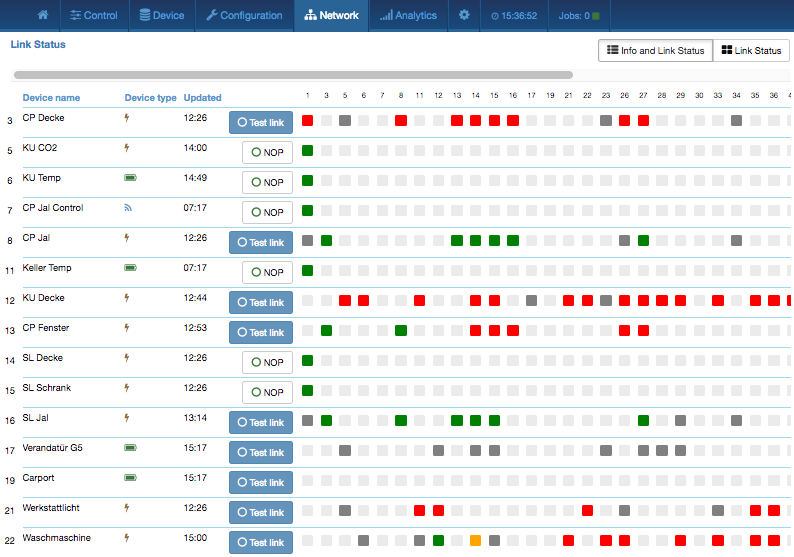
\includegraphics[width=0.9\textwidth]{pngs/cap7/eui26.png}
\caption{Link Status}
\label{eui26}
\end{center}
\end{figure}

The link status map, as shown in Figure \ref{eui26}, summarizes the device-specific link 
status information from the configuration sections.

The following colors are used:

\begin{itemize}
\item grey: untested
\item green: good quality
\item yellow: reasonable quality
\item red: link quality insufficient
\end{itemize}

The links from one device can be retested using the \keystroke{Test link} button. However, please 
keep in mind that this process may take several minutes to complete.
For devices that do not offer a link status function in their firmware, there is a simple 
connection test to the \zway controller using a ``NOP.’’ Please note that this function 
does not test a direct wireless connection but the route to the controller only.

\subsection{Controller Info}

\begin{figure}
\begin{center}
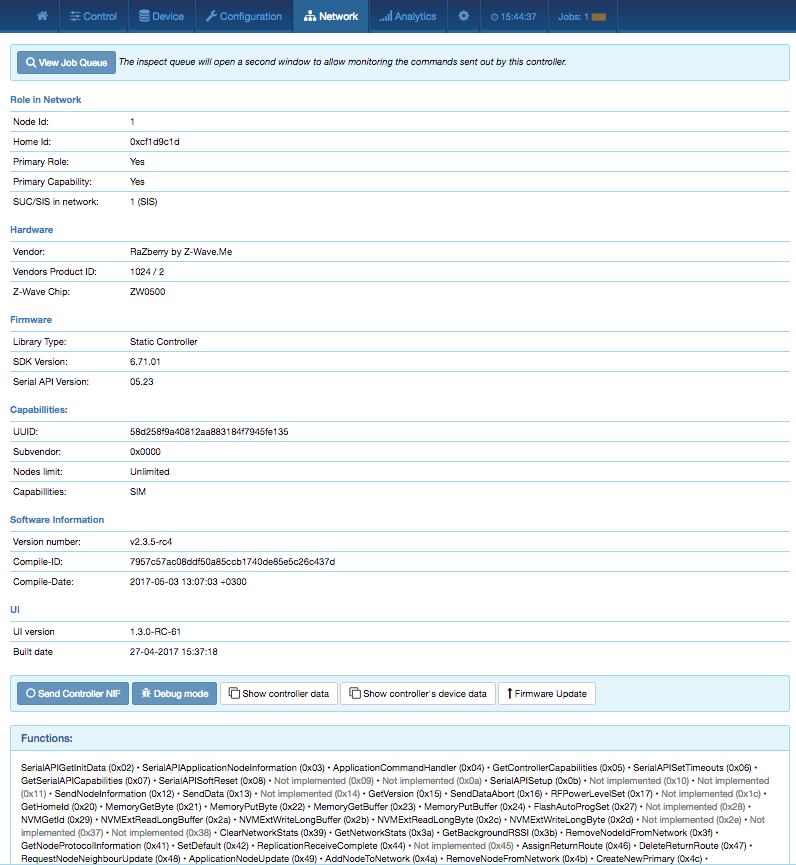
\includegraphics[width=0.9\textwidth]{pngs/cap7/eui27.png}
\caption{Controller Info}
\label{eui27}
\end{center}
\end{figure}

This menu item as shown in Figure \ref{eui27} provides some internal and very technical 
information about the \zway controller software, hardware, and firmware. The different 
submenu items are self-explaining.

Some buttons allow special maintenance functions:

\begin{itemize}

\item \keystroke{View Job Queue}: This button opens a new tab with a list of all wireless jobs in 
the system. For more information about this, please refer to Chapter \ref{jobqueue}. 
This is needed for debugging purposes only.
\item \keystroke{Send Controller NIF}: Sends out the Node Information Frame of the \zway controller. 
This is needed for debugging purposes only.
\item \keystroke{Debug Mode}: When active this button is shown in green. Active debugging unlocks 
some special function embedded in the rest of the Expert User Interface. Among them is the 
user interface to edit so-called ``Postfix Records.’’ The postfix function allows changing 
device capabilities after the device interview. Typical postfix entries suppress certain 
functions that are announced by the Node Information Frame of certain command classes but 
not or wrongly implemented. Postfix is also used to rename certain functions to more 
meaningful terms. Post fix entries are typically created during device testing.
\item \keystroke{Show controller data} and \keystroke{Show controller's device data}: The controller is a 
special node in the network but still a node. Therefore, buttons allow accessing the device 
specific data of the controller and issue a Node Information Frame. A third button gives 
access to the controller specific data. Most of these data is only relevant to developers.

\item \keystroke{Firmware Update}: This function allows updating the function of the \zwave 
transceiver used by \zway. Only valid update files will be offered. It is possible to 
add so-called tokens. These is a special string used to identify special function 
firmware or beta firmware. They are sued to make sure that this special firmware is only 
available to those that really need, e.g. for testing.
\end{itemize}


The last block of the dialog shows the availability of the function calls on the serial 
API between the \zwave transceiver and \zway. ``Not implemented’’ means that \zway is 
either not knowing about the function indicated by the function ID or does not make any 
use of it. A red function call ID or name indicated that \zway can use this function, but 
the transceiver’s firmware did not report to offer this service.

Annex \ref{FunctionClasses} gives a full overview of the Functions used and supported by \zway .

\subsection{Basic Set Handling}

Z-Wave protocol defines a minimal level of interoperability via Basic
Command Class. Most devices do act on \texttt{Basic Set} commands mapping it
to \texttt{Switch Binary Set} or \texttt{Thermostat Mode Set} or some other.
Z-Way is able to control other devices using speical Command Classes or
using Basic Set.

Z-Way is handling incoming \texttt{Basic Set} and creates a virtual device that
reflects the state of the last \texttt{Basic Set} command recieved. This
allows to work with old devices that do not send \texttt{Reports} or
\texttt{Central Scene Notification} to the LifeLine association group. Z-Way is
ignoring \texttt{Basic Get} commands.

\subsection{Security Considerations}

Z-Way supports both Security S2 and Security S0 protocols and implements
very strict security rules. See Table \ref{c7:security} for more
information.

\begin{table}
\begin{tabular}{|p{0.19\textwidth}|p{0.27\textwidth}|p{0.27\textwidth}|p{0.27\textwidth}|}
\hline
\textbf{Negociated security} & \textbf{Unsecure NIF} & \textbf{Security S0 NIF} & \textbf{Security S2 NIF} \\
\hline
No or failed security &
 \begin{tabular}{l}
  ZWavePlusInfo \\
  Version \\
  MultiCmd \\
  Security \\
  SecurityS2 \\
  Supervision \\
  ManufacturerSpecific \\
  NodeNaming \\
  ApplicationStatus \\
  CRC16 \\
  PowerLevel \\
  Association \\
  AssociationGroupInformation \\
  MultiChannelAssociation \\
  DeviceResetLocally \\
  TransportService \\
  InclusionController
 \end{tabular}
 & - & - \\
\hline
Security S0 &
 \begin{tabular}{l}
  ZWavePlusInfo \\
  MultiCmd \\
  Security \\
  SecurityS2 \\
  Supervision \\
  NodeNaming \\
  ApplicationStatus \\
  CRC16 \\
  PowerLevel \\
  AssociationGroupInformation \\
  DeviceResetLocally \\
  TransportService \\
  InclusionController
 \end{tabular}
 &
 \begin{tabular}{l}
  Version \\
  MultiCmd \\
  ManufacturerSpecific \\
  NodeNaming \\
  ApplicationStatus \\
  CRC16 \\
  PowerLevel \\
  Association \\
  AssociationGroupInformation \\
  MultiChannelAssociation \\
  DeviceResetLocally \\
  InclusionController
 \end{tabular}
 & - \\
\hline
Security S2 &
 \begin{tabular}{l}
  ZWavePlusInfo \\
  SecurityS2 \\
  Supervision \\
  TransportService
 \end{tabular}
 & - &
 \begin{tabular}{l}
  Version \\
  MultiCmd \\
  ManufacturerSpecific \\
  NodeNaming \\
  ApplicationStatus \\
  CRC16 \\
  PowerLevel \\
  Association \\
  AssociationGroupInformation \\
  MultiChannelAssociation \\
  DeviceResetLocally \\
  InclusionController
 \end{tabular}
 \\
\hline
\end{tabular}
\caption{Supported Command Classes depending on the security level negociated}
\label{c7:security}
\end{table}

\section {Analytics}

The analytics menu offers functions to troubleshoot a \zwave network. Details about the 
dialogs are provided in Chapter \ref{c5:cit}.


\section {Setup}

The setup dialog offers various options to adapt the behavior of the \zweui:

\begin{itemize}
\item Language: Pick your user interface language by clicking on one of the flags.
\item System Settings: This option allows setting the date format and the time zone.
\item Report Problem: This option allows reporting user interface bugs. Please note that 
the form will transmit the test, he option email address for questions and answers plus 
some internal version and status information.
\end{itemize}

\section{Job Queue}
\label{jobqueue}

\begin{figure}
\begin{center}
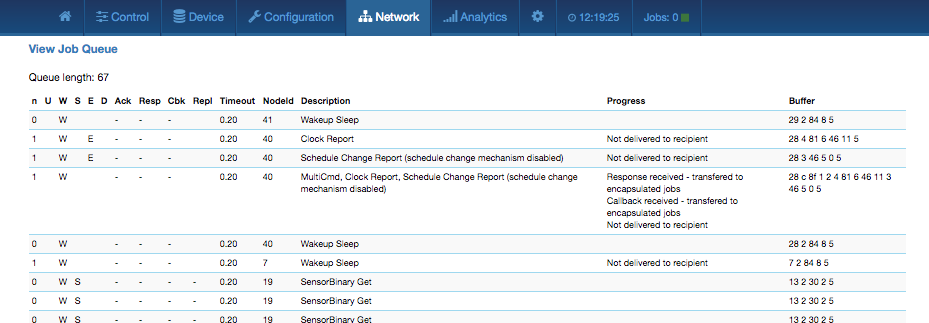
\includegraphics[width=0.9\textwidth]{pngs/cap7/eui28.png}
\caption{Job Queue}
\label{eui28}
\end{center}
\end{figure}

The job queue, as shown in Figure \ref{eui28}, offers some deep insight into the dynamics 
of the controller software. It visualizes the (wireless) task execution of the system. 
Every communication attempt of the controller is queued and then handed over to the \zwave 
chip for execution. The list shows the jobs pending and the jobs that are completed or failed.

A legend informs about the meaning of the different flags n, U, D, E, S, and W. The timeout 
value counts back from 20 seconds once the job was sent. Even when it is completed, the 
job will stay in the queue marked as done (D) for some more time to allow inspection. The 
target node ID, a description of the communication message, information about the process,
 and the real bytes of the message are shown as well.
